\documentclass[a4paper, 16pt]{article}
\usepackage[utf8]{inputenc}
\usepackage[english, russian]{babel} 
\usepackage[left=20mm, top=20mm, right=20mm,
 bottom=20mm, head=1mm, foot=1mm]{geometry}
\usepackage{tikz} 
\usepackage{amsmath, amsfonts, amssymb}
\usepackage{graphicx}
\usepackage{fancybox, fancyhdr}
\usepackage{hyperref}
\usepackage{listings}
\usepackage{caption}
\usepackage{subcaption}
\usepackage{xcolor}
\pagestyle{fancy}
\fancyhf{}
\fancyhead[L]{Лабораторная работа №2}
\fancyhead[R]{Частотные методы}
\fancyfoot[C]{\thepage}
\graphicspath{{images/}}
\usetikzlibrary{patterns}
\definecolor{LightGray}{gray}{0.95}
\lstdefinestyle{pycode}{
    language=Python,
    basicstyle=\footnotesize\ttfamily,
    numbers=left,
    numberstyle=\tiny\color{gray},
    stepnumber=1,
    numbersep=5pt,
    backgroundcolor=\color{LightGray},
    showspaces=false,
    showstringspaces=false,
    showtabs=false,
    tabsize=4,
    captionpos=b,
    breaklines=true,
    breakatwhitespace=false,
    frame=single,
    rulecolor=\color{black},
    linewidth=\linewidth,
    keywordstyle=\color{red}\bfseries,
    commentstyle=\color{green!40!black},
    stringstyle=\color{purple},
    escapeinside={\%*}{*)},
    xleftmargin=0pt,
    framexleftmargin=0pt,
    framexrightmargin=0pt
}
\lstset{style=pycode}
\hypersetup{
    colorlinks=true,
    linkcolor=blue,
    filecolor=magenta,      
    urlcolor=cyan,
    pdftitle={contents setup},
    pdfpagemode=FullScreen,
}
\allowdisplaybreaks
\DeclareMathOperator{\sinc}{sinc}
\newcommand{\frc}[2]{\raisebox{2pt}{$#1$}\big/\raisebox{-3pt}{$#2$}}

\begin{document}
\begin{titlepage}

    \begin{center}
    \vfill
    
    Федеральное государственное автономное образовательное учреждение высшего образования\\
    «Национальный Исследовательский Университет ИТМО»\ \\
    
    \vfill
    {\large\bf ЛАБОРАТОРНАЯ РАБОТА №2\\
        ПО ПРЕДМЕТУ «ЧАСТОТНЫЕ МЕТОДЫ»\\
        ПО ТЕМЕ «ПРЕОБРАЗОВАНИЕ ФУРЬЕ»}
    \vfill
        
    \begin{flushright}
        \begin{minipage}{.45\textwidth}
        {
            \hbox{Лектор: Перегудин А. А.}
            \hbox{Практик: Пашенко А. В.}
            \hbox{Студент: Румянцев А. А.}
            \hbox{Поток: ЧАСТ.МЕТ. 1.3}
            \hbox{}
            \hbox{Факультет: СУиР}
            \hbox{Группа: R3241}
        }
        \end{minipage}
    \end{flushright}
    
    \vfill
            
    Санкт-Петербург\\
    2024
    \end{center}
    \end{titlepage}
    \setlength{\parskip}{1.5mm}
    
    \tableofcontents

    \newpage
    \section{Введение}
    \noindent В заданиях 1 и 2 используется унитарное преобразование Фурье к угловой частоте $\omega$.\
    Подсчет Фурье- -образа производится по формуле ниже
    $$
    \hat{f}\left(\omega\right)=\dfrac{1}{\sqrt{2\pi}}\int\limits_{-\infty}^{\infty}f(t)e^{-i\omega t}\,dt
    $$
    

    \noindent В задании 3 используется преобразование Фурье к обыкновенной частоте $\nu$. В общем\
    виде формула имеет вид
    $$
    \hat{f}\left(\nu\right)=\int\limits_{-\infty}^{\infty}f\left(t\right)e^{-2\pi i \nu t}\,dt
    $$


    \noindent Для проверки равенства Парсеваля используется формула ниже
    $$
    \left|\left|f\right|\right|_2=||\hat{f}||_2,
    $$
    \noindent где $||f||_2$ -- вторая норма заданной фукнции, $||\hat{f}||_2$ -- вторая норма
    Фурье-образа функции $f$. Для нахождения нормы используются формулы, представленные ниже
    $$
    ||f(t)||_2=\sqrt{\int\limits_{a}^{b}f(t)\cdot f^{*}(t)\,dt},\,\,\,\,\,\,\,\,||\hat{f}(\omega)||_2=\sqrt{\int\limits_{a}^{b}\hat{f}(\omega)\cdot \hat{f}^{*}(\omega)\,d\omega}
    $$


    \noindent Все графики строятся программой, написанной на языке программирования python. В 1 и 2 заданиях\
    используется библиотека sympy, в задании 3 numpy и matplotlib. По ходу отчета приводится код для каждого задания.
    Для всех интегралов и графиков есть место с общими переменными и значениями -- файл static.py. Основные используемые
    данные приведены ниже
    \begin{lstlisting}[label=static, caption=Основные данные из файла static.py]
    from sympy import Symbol, Piecewise, Abs, sinc, E, oo

    t = Symbol('t')
    omega = Symbol('omega')

    interval = [-oo, oo]

    a_b_pars = [(1, 2), (2, 3), (3, 4)]
    consts = [-1, 0.5, 1]
    colors_strs = ['red', 'purple', 'blue', 'cyan'] 
    \end{lstlisting}


    \noindent В этом файле программно заданы функции, графики которых приводятся по ходу отчета. Также они необходимы
    для нахождения их Фурье-образа
    \begin{lstlisting}[label=funcs, caption=Программно заданные функции для заданий 1 и 2]
    def rectangular_function(a, b):
        return Piecewise((a, Abs(t) <= b), (0, Abs(t) > b))

    def triangular_function(a, b):
        return Piecewise((a - Abs(a * t / b), Abs(t) <= b), (0, Abs(t) > b))

    def cardinal_sinus(a, b):
        return a * sinc(b * t)
    
    def gaussian_function(a, b):
        return a * E ** (-b * t ** 2)
    
    def double_attenuation(a, b):
        return a * E ** (-b * Abs(t))
    \end{lstlisting}


    \section{Задание 1. Вещественное}
    \subsection{Прямоугольная функция}
    \noindent Рассмотрим прямоугольную функцию следующего вида
    $$
    f(t)=
    \begin{cases}
        a, & \left|t\right|\leq b,\\
        0, & \left|t\right|>b.
    \end{cases}
    $$


    % аналитическое выражение с выводом


    \noindent Рассмотрим программу. Сначала задается функция, принимающая параметры $a\text{ и }b$, после чего методом build\_{f}\_{t} строится график $f(t)$.
    На строке 10 приведен пример использования кода
    \begin{lstlisting}[label=f_t_rect, caption=Программа для построения графика прямоугольной функции]
    def build_f_t(f_t, clr, lbl):
        if (lbl == None):
            plot(f_t, line_color=clr, xlabel=r'$t$', ylabel=r'$f(t)$')
        else:
            plot(f_t, line_color=clr, xlabel=r'$t$', ylabel=r'$f(t)$', label=lbl, legend=True)

    build_f_t(rectangular_function(1, 2), 'red', None)
    \end{lstlisting}


    \noindent Построенные графики $f(t)$ для нескольких значений параметров $a,b>0$ расположены ниже
    \begin{figure}[htbp]
        \centering
        \begin{subfigure}{0.3\textwidth}
            \centering
            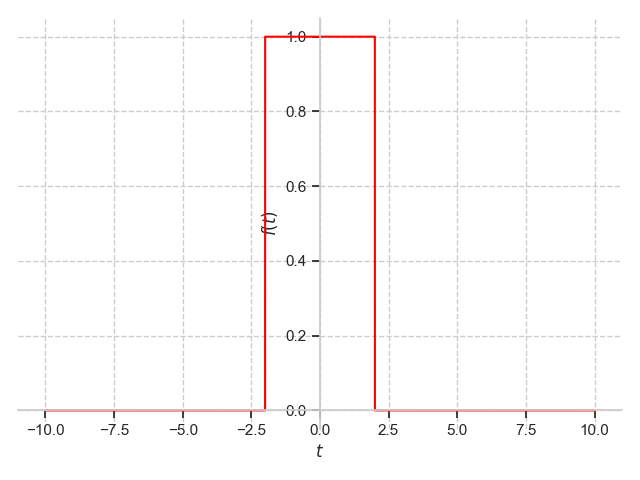
\includegraphics[width=\linewidth]{rectf_a=1_b=2.png}
            \caption{$a=1,\,\,b=2$}
            \label{fig:rectf_1}
        \end{subfigure}
        \hfill
        \begin{subfigure}{0.3\textwidth}
            \centering
            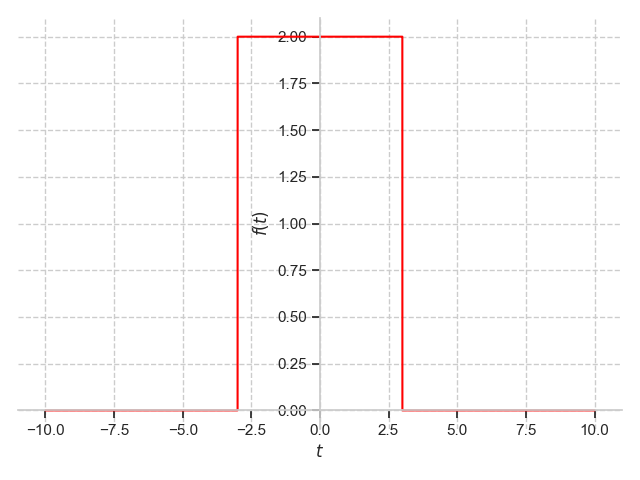
\includegraphics[width=\linewidth]{rectf_a=2_b=3.png}
            \caption{$a=2,\,\,b=3$}
            \label{fig:rectf_2}
        \end{subfigure}
        \hfill
        \begin{subfigure}{0.3\textwidth}
            \centering
            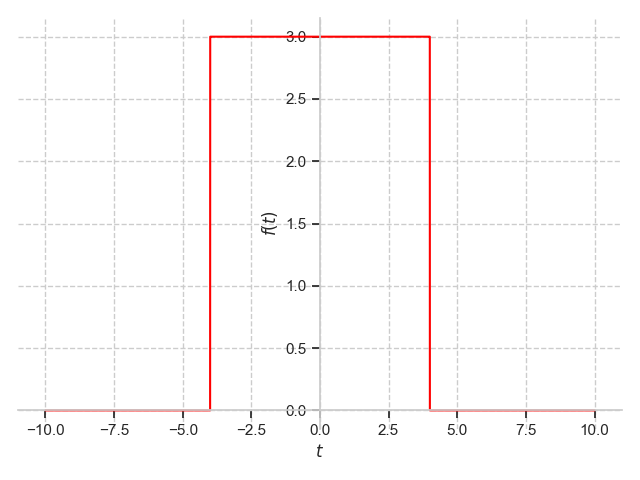
\includegraphics[width=\linewidth]{rectf_a=3_b=4.png}
            \caption{$a=3,\,\,b=4$}
            \label{fig:rectf_3}
        \end{subfigure}
        \caption{Прямоугольные функции при различных значениях $a$ и $b$}
        \label{fig:rectfs}
    \end{figure}


    \noindent Рассмотрим программу. Методом find\_{fimg} находится Фурье-образ заданной функции. Далее методом build\_{fimg2}
    строится график Фурье-образа. На 16-17 строчках находится пример использования кода
    \begin{lstlisting}[label=fimg_rect, caption=Программа для построения графика Фурье-образа некоторой функции $f(t)$]
    def find_fimg(f_t, lim1, lim2):
        integrand = f_t * E ** (-I * omega * t)

        result = integrate(integrand, (t, lim1, lim2))
        return coeff * result

    def build_fimg2(fimg, clr, lbl):
        if (lbl == None):
            plot(fimg, line_color=clr,
                 xlabel=r'$\omega$', ylabel=r'$c(\omega)$')
        else:
            plot(fimg, line_color=clr,
                 xlabel=r'$\omega$', ylabel=r'$c(\omega)$',
                 label=lbl, legend=True)
    
    rectfimg = find_fimg(rectangular_function, -oo, oo)
    build_fimg2(rectfimg, 'purple', None)
    \end{lstlisting}


    \noindent Построенные графики $\hat{f}\left(\omega\right)$ для тех же значений $a$ и $b$ расположены ниже
    \begin{figure}[htbp]
        \centering
        \begin{subfigure}{0.3\textwidth}
            \centering
            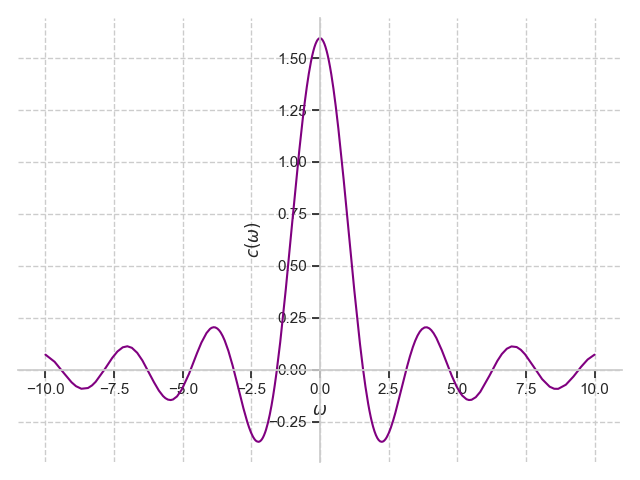
\includegraphics[width=\linewidth]{rectfimg_a=1_b=2.png}
            \caption{$a=1,\,\,b=2$}
            \label{fig:rectfimg_1}
        \end{subfigure}
        \hfill
        \begin{subfigure}{0.3\textwidth}
            \centering
            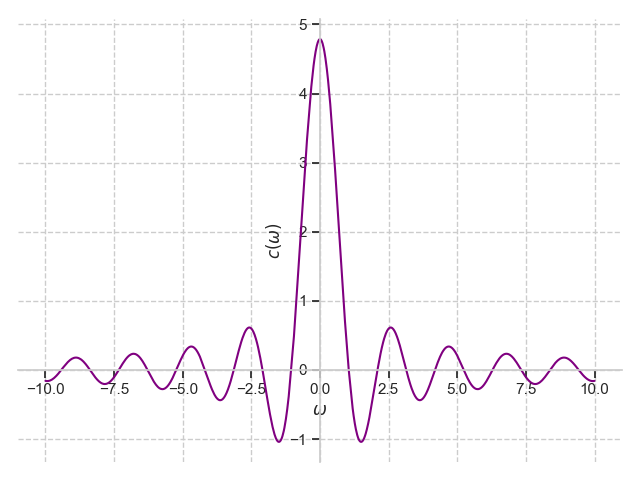
\includegraphics[width=\linewidth]{rectfimg_a=2_b=3.png}
            \caption{$a=2,\,\,b=3$}
            \label{fig:rectfimg_2}
        \end{subfigure}
        \hfill
        \begin{subfigure}{0.3\textwidth}
            \centering
            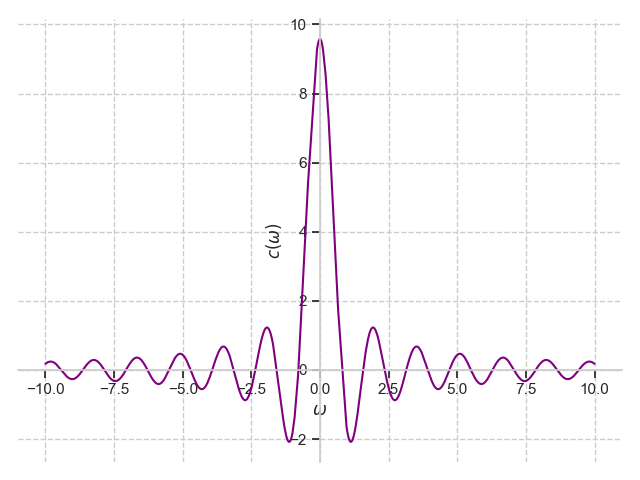
\includegraphics[width=\linewidth]{rectfimg_a=3_b=4.png}
            \caption{$a=3,\,\,b=4$}
            \label{fig:rectfimg_3}
        \end{subfigure}
        \caption{Фурье-образы прямоугольных функций при различных значениях $a$ и $b$}
        \label{fig:rectfimgs}
    \end{figure}


    % анализ графиков и ответы на вопросы


    \noindent Рассмотрим программу. Методом find\_{norm2} находится вторая норма переданной функции.
    Метод \\find\_{parseval} считает левую и правую части равенства Парсеваля. Пример использования кода
    расположен на 13-14 строчках листинга ниже
    \begin{lstlisting}[label=pars_rectf, caption=Программа для нахождения левой и правой сторон равенства Парсеваля]
    def find_norm2(f, lim1, lim2, var):
        integrand = f * conjugate(f)

        result = integrate(integrand, (var, lim1, lim2)).evalf()
        return sqrt(result).evalf()

    def find_parseval(f, fimg, lim1, lim2):
        pleft = find_norm2(f, lim1, lim2, t)
        pright = find_norm2(fimg, lim1, lim2, omega)

        return pleft, pright

    pl, pr = find_parseval(rectangular_function, rectfimg, -oo, oo)
    print(f'p_{1}: {pl} ?= {pr}')
    \end{lstlisting}


    \noindent Программа вывела в консоль результаты, представленные ниже
    \begin{lstlisting}[label=pres_rectf, caption=Результат выполнения программы для вычисления равенства Парсеваля]
    p_1: 2.00000000000000 ?= 2.0 + 0.e-114*I  
    p_2: 4.89897948556636 ?= 4.89897948556636 + 0.e-114*I 
    p_3: 8.48528137423857 ?= 8.48528137423857 + 0.e-114*I
    \end{lstlisting}


    \noindent Мнимыми частями в правой части равенства Парсеваля пренебрежем вследствие их стремления к нулю. В таком случае равенство Парсеваля выполняется, что можно объяснить тем, что интеграл позволяет
    рассмотреть норму непрерывно на заданном промежутке, а ряд только дискретно, вследствие чего теряются какие-то члены ряда,
    которых не хватает для выполнения равенства Парсеваля


    \subsection{Треугольная функция}
    \noindent Рассмотрим треугольную функцию следующего вида
    $$
    f(t)=
    \begin{cases}
        a-\left|\dfrac{at}{b}\right|, & \left|t\right|\leq b,\\
        0, & \left|t\right|>b.
    \end{cases}
    $$


    % аналитическое выражение с выводом


    \noindent Для построения графиков треугольной функции сначала задается необходимая функция,
    после используется код, приведенный в пункте 2.1 для прямоугольной функции
    \begin{lstlisting}[label=triangf, caption=Программно заданная треугольная функция]
    null
    \end{lstlisting}


    \noindent Построенные графики $f(t)$ для нескольких значений параметров $a,b>0$ расположены ниже
    \begin{figure}[htbp]
        \centering
        \begin{subfigure}{0.3\textwidth}
            \centering
            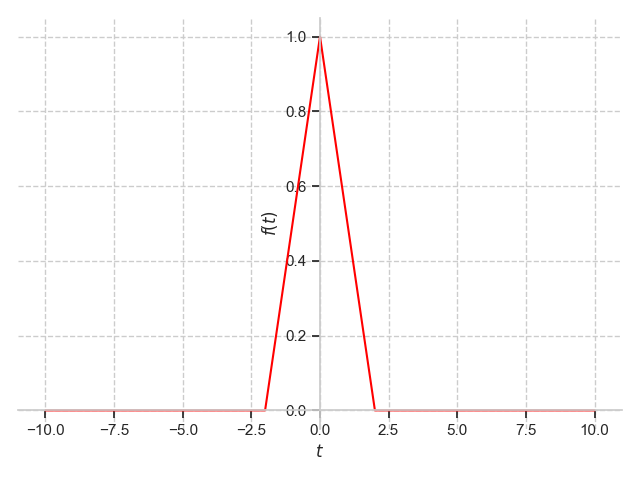
\includegraphics[width=\linewidth]{trif_a=1_b=2.png}
            \caption{$a=1,\,\,b=2$}
            \label{fig:triangf_1}
        \end{subfigure}
        \hfill
        \begin{subfigure}{0.3\textwidth}
            \centering
            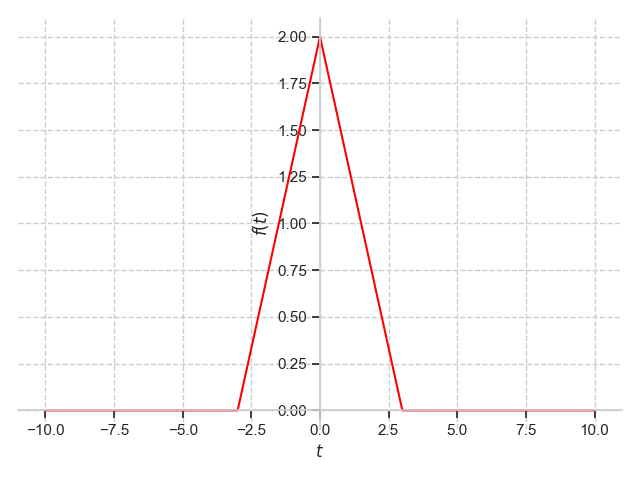
\includegraphics[width=\linewidth]{trif_a=2_b=3.png}
            \caption{$a=2,\,\,b=3$}
            \label{fig:triangf_2}
        \end{subfigure}
        \hfill
        \begin{subfigure}{0.3\textwidth}
            \centering
            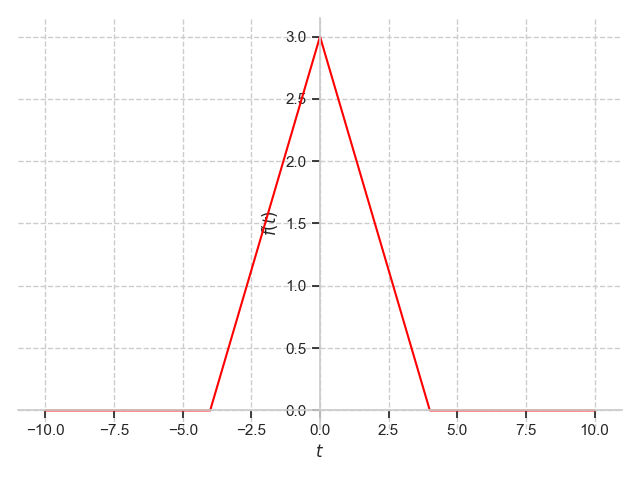
\includegraphics[width=\linewidth]{trif_a=3_b=4.png}
            \caption{$a=3,\,\,b=4$}
            \label{fig:triangf_3}
        \end{subfigure}
        \caption{Треугольные функции при различных значениях $a$ и $b$}
        \label{fig:triangfs}
    \end{figure}


    \noindent Построенные графики $\hat{f}\left(\omega\right)$ для тех же значений $a$ и $b$ расположены ниже
    \begin{figure}[htbp]
        \centering
        \begin{subfigure}{0.3\textwidth}
            \centering
            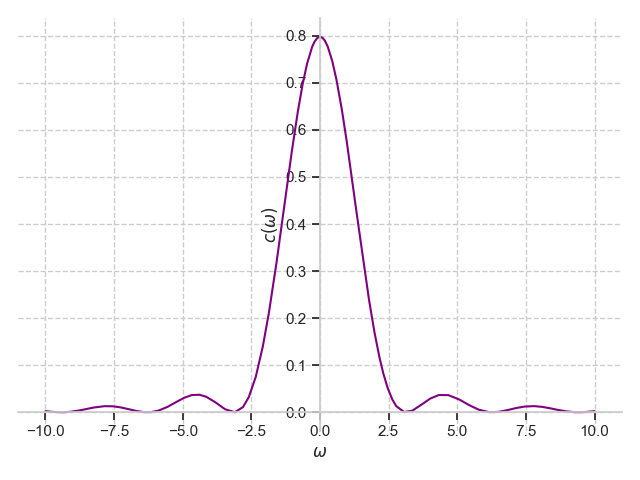
\includegraphics[width=\linewidth]{trifimg_a=1_b=2.png}
            \caption{$a=1,\,\,b=2$}
            \label{fig:trifimg_1}
        \end{subfigure}
        \hfill
        \begin{subfigure}{0.3\textwidth}
            \centering
            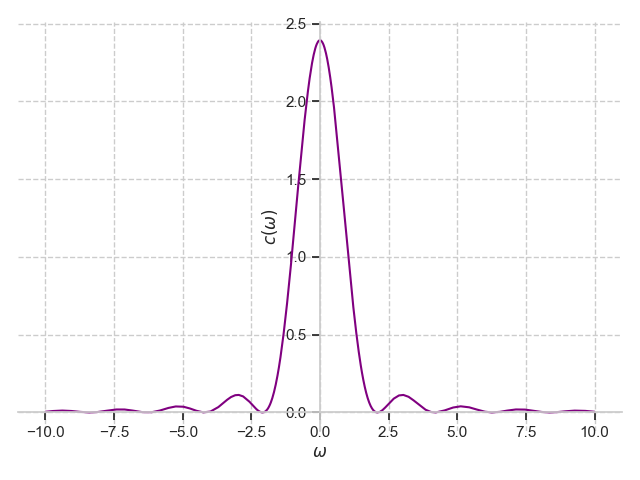
\includegraphics[width=\linewidth]{trifimg_a=2_b=3.png}
            \caption{$a=2,\,\,b=3$}
            \label{fig:trifimg_2}
        \end{subfigure}
        \hfill
        \begin{subfigure}{0.3\textwidth}
            \centering
            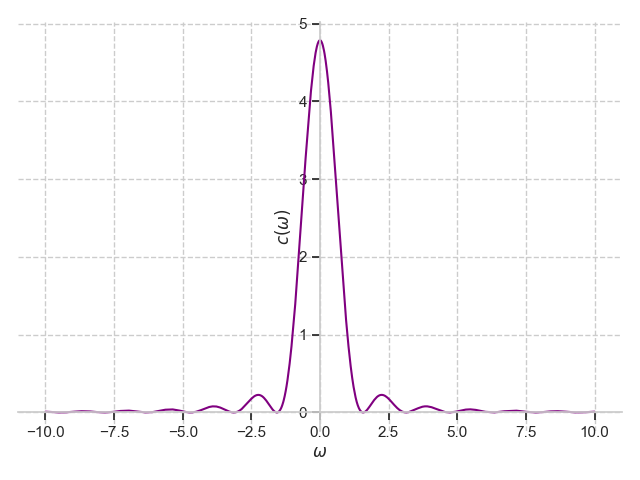
\includegraphics[width=\linewidth]{trifimg_a=3_b=4.png}
            \caption{$a=3,\,\,b=4$}
            \label{fig:trifimg_3}
        \end{subfigure}
        \caption{Фурье-образы треугольных функций при различных значениях $a$ и $b$}
        \label{fig:trifimgs}
    \end{figure}


    % анализ графиков и ответы на вопросы


    \noindent Проверим программой выполнение равенства Парсеваля
    \begin{lstlisting}[label=parstrif, caption=Равенство Парсеваля для треугольных функций]
    p_1: 1.15470053837925 ?= 1.15470053837925
    p_2: 2.82842712474619 ?= 2.82842712474619
    p_3: 4.89897948556636 ?= 4.89897948556636
    \end{lstlisting}


    \noindent Равенство Парсеваля выполняется для треугольной функции


    \subsection{Кардинальный синус}
    \noindent Рассмотрим кардинальный синус следующего вида
    $$
    f(t)=a\cdot \sinc{(bt)}
    $$


    % аналитическое выражение


    \noindent Построенные графики $f(t)$ для нескольких значений параметров $a,b>0$ расположены ниже
    \begin{figure}[htbp]
        \centering
        \begin{subfigure}{0.3\textwidth}
            \centering
            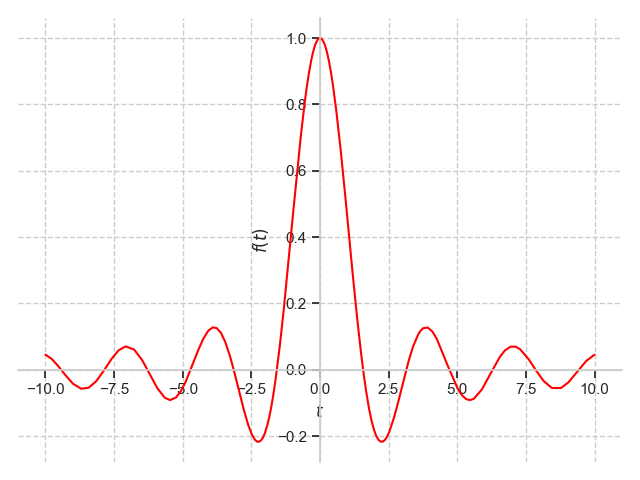
\includegraphics[width=\linewidth]{sinc_a=1_b=2.png}
            \caption{$a=1,\,\,b=2$}
            \label{fig:sinc_1}
        \end{subfigure}
        \hfill
        \begin{subfigure}{0.3\textwidth}
            \centering
            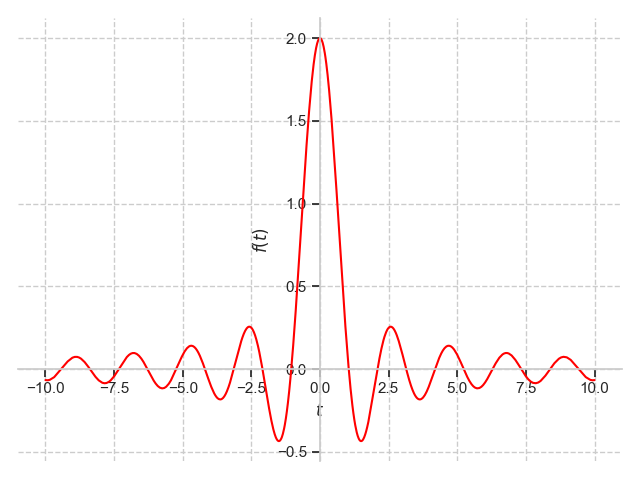
\includegraphics[width=\linewidth]{sinc_a=2_b=3.png}
            \caption{$a=2,\,\,b=3$}
            \label{fig:sinc_2}
        \end{subfigure}
        \hfill
        \begin{subfigure}{0.3\textwidth}
            \centering
            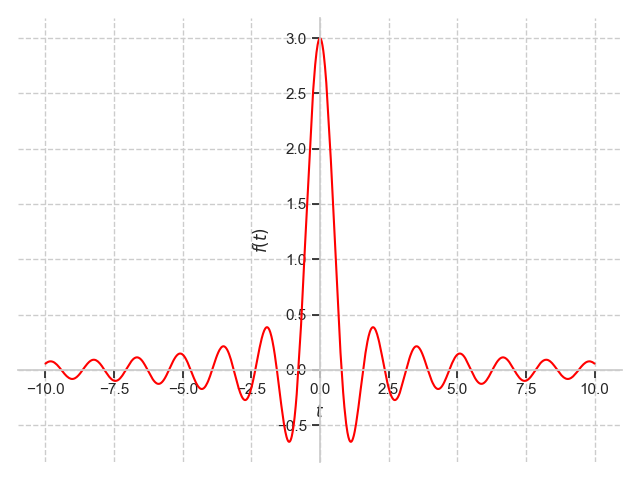
\includegraphics[width=\linewidth]{sinc_a=3_b=4.png}
            \caption{$a=3,\,\,b=4$}
            \label{fig:sinc_3}
        \end{subfigure}
        \caption{Кардинальные синусы при различных значениях $a$ и $b$}
        \label{fig:sincs}
    \end{figure}


    \noindent Построенные графики $\hat{f}\left(\omega\right)$ для тех же значений $a$ и $b$ расположены ниже
    \begin{figure}[htbp]
        \centering
        \begin{subfigure}{0.3\textwidth}
            \centering
            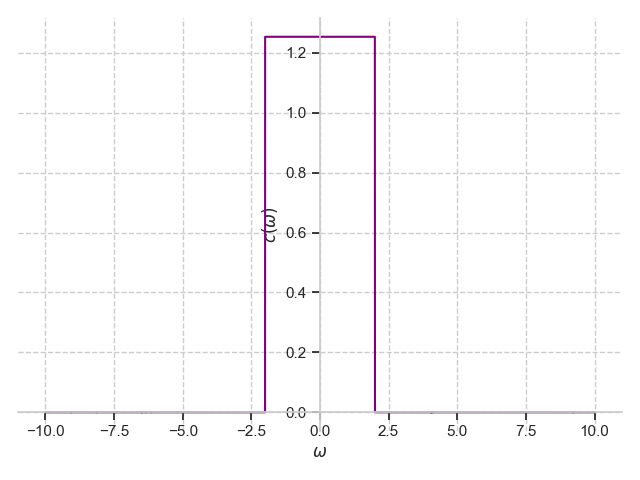
\includegraphics[width=\linewidth]{sincfimg_a=1_b=2.png}
            \caption{$a=1,\,\,b=2$}
            \label{fig:sincfimg_1}
        \end{subfigure}
        \hfill
        \begin{subfigure}{0.3\textwidth}
            \centering
            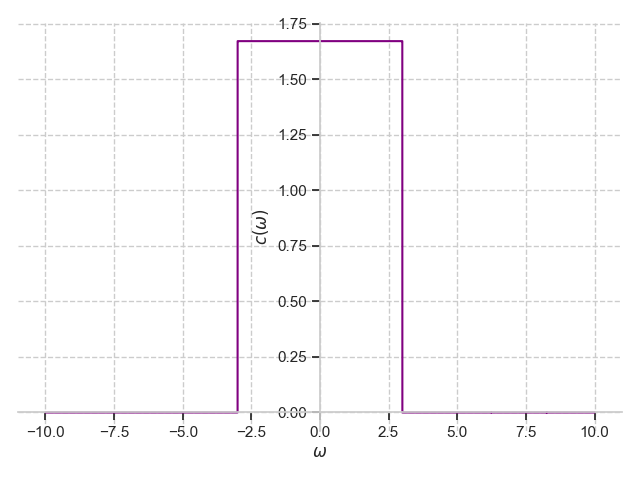
\includegraphics[width=\linewidth]{sincfimg_a=2_b=3.png}
            \caption{$a=2,\,\,b=3$}
            \label{fig:sincfimg_2}
        \end{subfigure}
        \hfill
        \begin{subfigure}{0.3\textwidth}
            \centering
            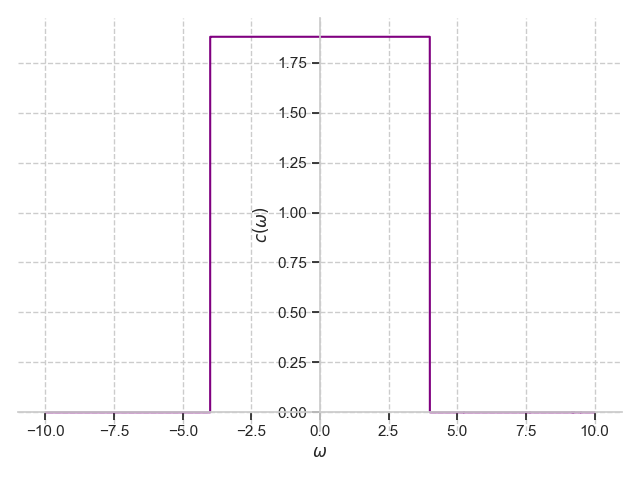
\includegraphics[width=\linewidth]{sincfimg_a=3_b=4.png}
            \caption{$a=3,\,\,b=4$}
            \label{fig:sincfimg_3}
        \end{subfigure}
        \caption{Фурье-образы кардинальных синусов при различных значениях $a$ и $b$}
        \label{fig:sincfimgs}
    \end{figure}


    % анализ графиков и ответы на вопросы


    \noindent Проверим программой выполнение равенства Парсеваля
    \begin{lstlisting}[label=pars_sinc, caption=Равенство Парсеваля для кардинальных синусов]
    p_1: 1.25331412734194 ?= 1.25331412734194
    p_2: 2.04665340503514 ?= 2.04665340503514
    p_3: 2.65868076577972 ?= 2.65868076577972
    \end{lstlisting}


    \noindent Результат программы показывает, что равенство Парсеваля выполняется для кардинального синуса


    \subsection{Функция Гаусса}
    \noindent Рассмотрим фукнцию Гаусса следующего вида
    $$
    f(t)=ae^{-bt^2}
    $$


    % аналитическое выражение


    \noindent Построенные графики $f(t)$ для нескольких значений параметров $a,b>0$ расположены ниже
    \begin{figure}[htbp]
        \centering
        \begin{subfigure}{0.3\textwidth}
            \centering
            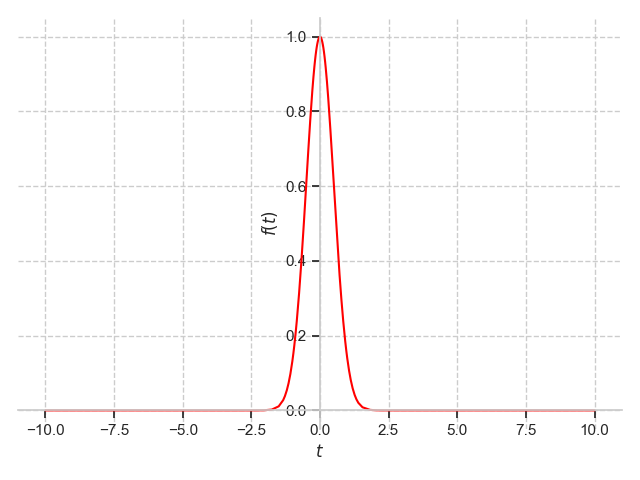
\includegraphics[width=\linewidth]{gaus_a=1_b=2.png}
            \caption{$a=1,\,\,b=2$}
            \label{fig:gaus_1}
        \end{subfigure}
        \hfill
        \begin{subfigure}{0.3\textwidth}
            \centering
            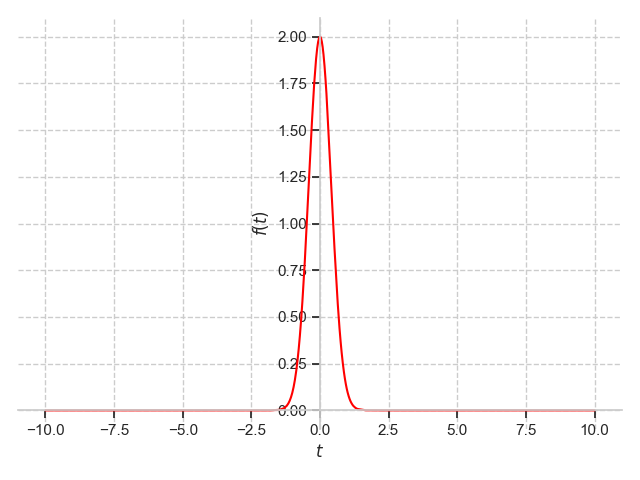
\includegraphics[width=\linewidth]{gaus_a=2_b=3.png}
            \caption{$a=2,\,\,b=3$}
            \label{fig:gaus_2}
        \end{subfigure}
        \hfill
        \begin{subfigure}{0.3\textwidth}
            \centering
            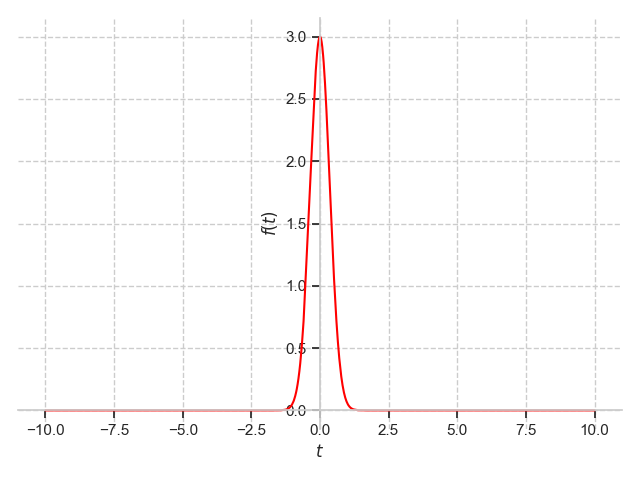
\includegraphics[width=\linewidth]{gaus_a=3_b=4.png}
            \caption{$a=3,\,\,b=4$}
            \label{fig:gaus_3}
        \end{subfigure}
        \caption{Функции Гаусса при различных значениях $a$ и $b$}
        \label{fig:gauss}
    \end{figure}


    \noindent Построенные графики $\hat{f}\left(\omega\right)$ для тех же значений $a$ и $b$ расположены ниже
    \begin{figure}[htbp]
        \centering
        \begin{subfigure}{0.3\textwidth}
            \centering
            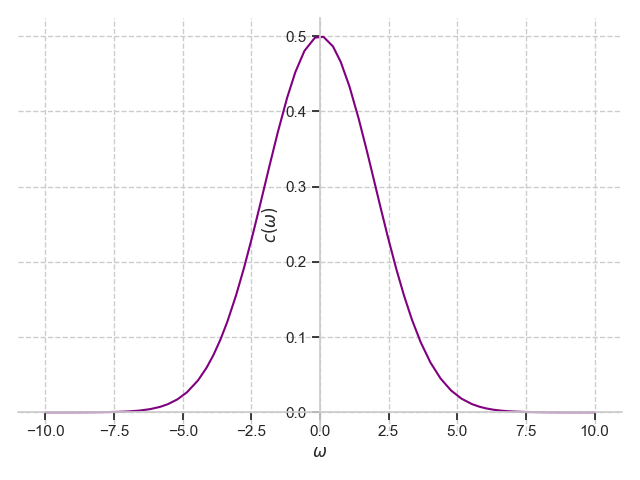
\includegraphics[width=\linewidth]{gausfimg_a=1_b=2.png}
            \caption{$a=1,\,\,b=2$}
            \label{fig:gausfimg_1}
        \end{subfigure}
        \hfill
        \begin{subfigure}{0.3\textwidth}
            \centering
            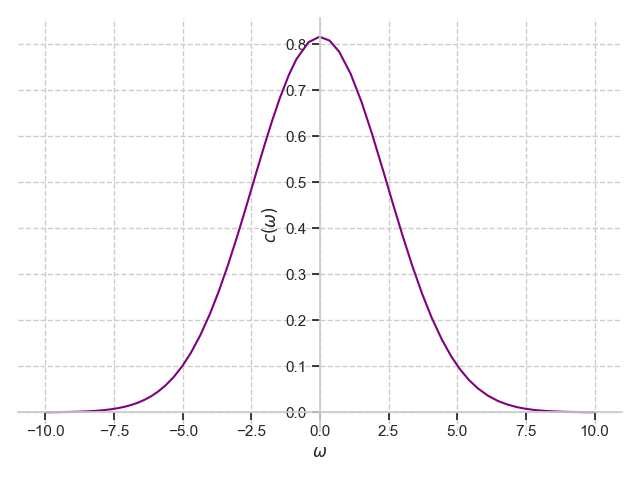
\includegraphics[width=\linewidth]{gausfimg_a=2_b=3.png}
            \caption{$a=2,\,\,b=3$}
            \label{fig:gausfimg_2}
        \end{subfigure}
        \hfill
        \begin{subfigure}{0.3\textwidth}
            \centering
            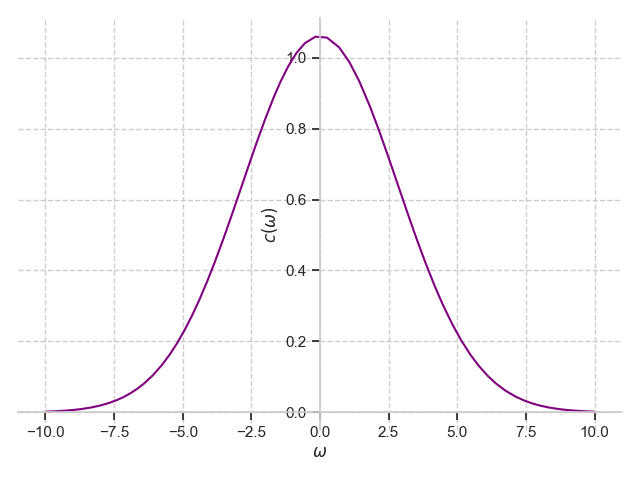
\includegraphics[width=\linewidth]{gausfimg_a=3_b=4.png}
            \caption{$a=3,\,\,b=4$}
            \label{fig:gausfimg_3}
        \end{subfigure}
        \caption{Фурье-образы функций Гаусса при различных значениях $a$ и $b$}
        \label{fig:gausfimgs}
    \end{figure}


    % анализ графиков и ответы на вопросы


    \noindent Проверим программой выполнение равенства Парсеваля
    \begin{lstlisting}[label=pars_gaus, caption=Равенство Парсеваля для функции Гаусса]
    p_1: 0.941396263776715 ?= 0.941396263776715
    p_2: 1.70129510027892 ?= 1.70129510027892
    p_3: 2.37485023062924 ?= 2.37485023062924
    \end{lstlisting}


    \noindent Результат говорит о выполнении равенства Парсеваля для фукнции Гаусса


    \subsection{Двустороннее затухание}
    \noindent Рассмотрим двустороннее затухание следующего вида
    $$
    f(t)=ae^{-b|t|}
    $$


    % аналитическое выражение и вывод


    \noindent Построенные графики $f(t)$ для нескольких значений параметров $a,b>0$ расположены ниже
    \begin{figure}[htbp]
        \centering
        \begin{subfigure}{0.3\textwidth}
            \centering
            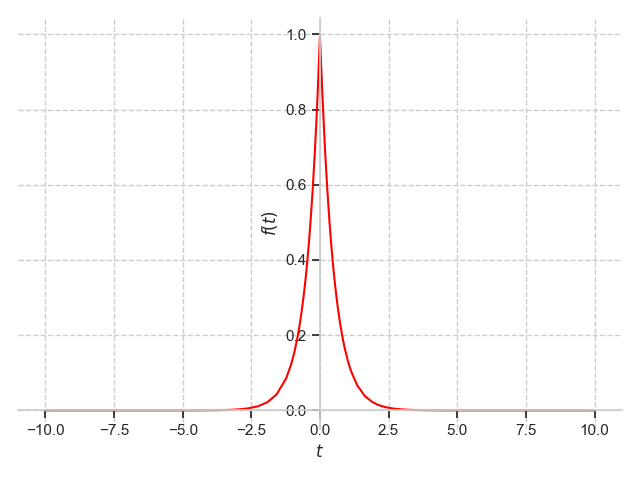
\includegraphics[width=\linewidth]{doat_a=1_b=2.png}
            \caption{$a=1,\,\,b=2$}
            \label{fig:doat_1}
        \end{subfigure}
        \hfill
        \begin{subfigure}{0.3\textwidth}
            \centering
            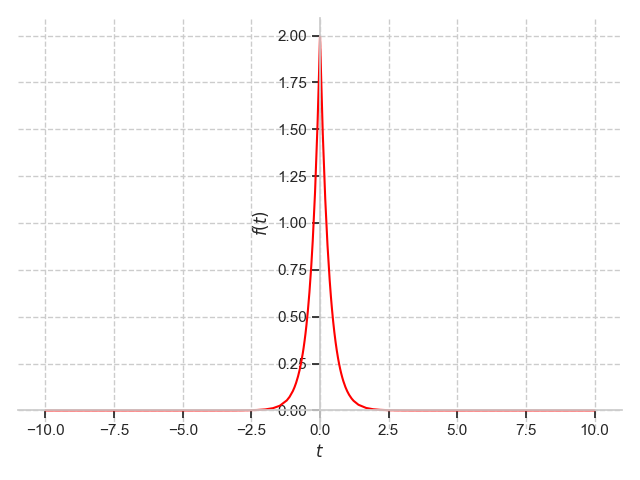
\includegraphics[width=\linewidth]{doat_a=2_b=3.png}
            \caption{$a=2,\,\,b=3$}
            \label{fig:doat_2}
        \end{subfigure}
        \hfill
        \begin{subfigure}{0.3\textwidth}
            \centering
            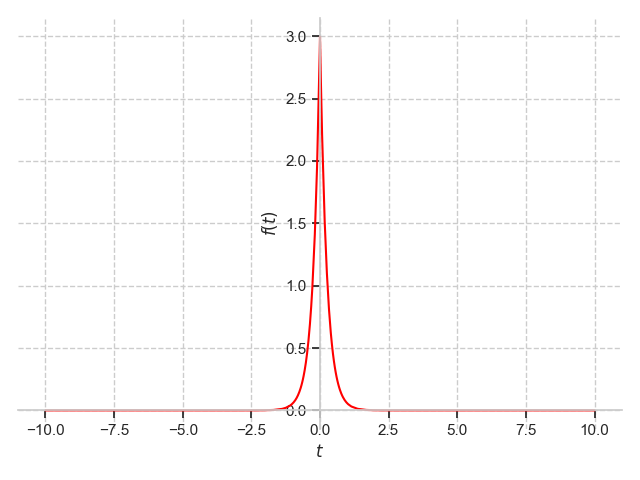
\includegraphics[width=\linewidth]{doat_a=3_b=4.png}
            \caption{$a=3,\,\,b=4$}
            \label{fig:doat_3}
        \end{subfigure}
        \caption{Двусторонние затухания при различных значениях $a$ и $b$}
        \label{fig:doats}
    \end{figure}


    \noindent Построенные графики $\hat{f}\left(\omega\right)$ для тех же значений $a$ и $b$ расположены ниже
    \begin{figure}[htbp]
        \centering
        \begin{subfigure}{0.3\textwidth}
            \centering
            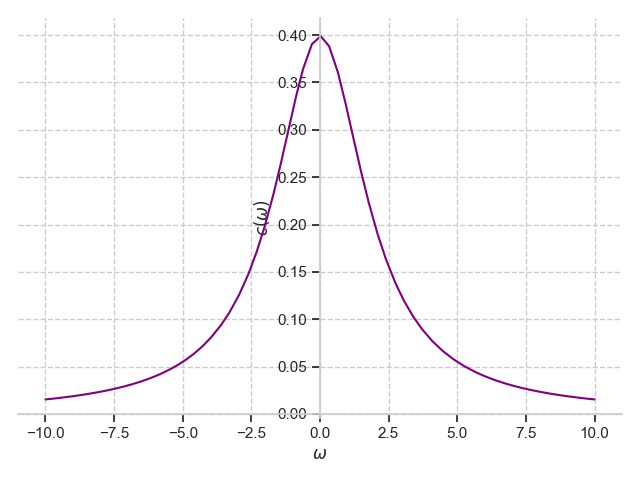
\includegraphics[width=\linewidth]{doatfimg_a=1_b=2.png}
            \caption{$a=1,\,\,b=2$}
            \label{fig:doatfimg_1}
        \end{subfigure}
        \hfill
        \begin{subfigure}{0.3\textwidth}
            \centering
            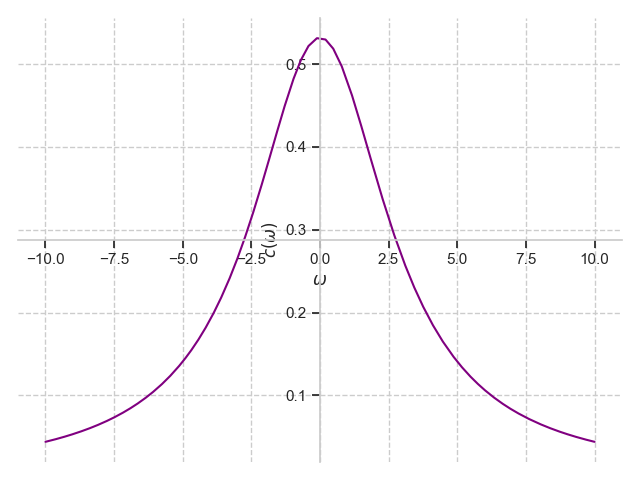
\includegraphics[width=\linewidth]{doatfimg_a=2_b=3.png}
            \caption{$a=2,\,\,b=3$}
            \label{fig:doatfimg_2}
        \end{subfigure}
        \hfill
        \begin{subfigure}{0.3\textwidth}
            \centering
            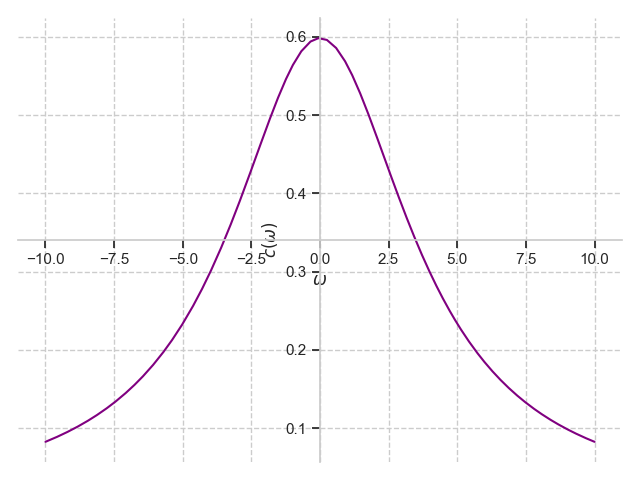
\includegraphics[width=\linewidth]{doatfimg_a=3_b=4.png}
            \caption{$a=3,\,\,b=4$}
            \label{fig:doatfimg_3}
        \end{subfigure}
        \caption{Фурье-образы двусторонних затуханий при различных значениях $a$ и $b$}
        \label{fig:doatfimgs}
    \end{figure}


    % анализ графиков и ответы на вопросы


    \noindent Проверим программой выполнение равенства Парсеваля
    \begin{lstlisting}[label=pars_doat, caption=Равенство Парсеваля для функции Гаусса]
    p_1: 0.700601299282005 ?= 0.700601299282005
    p_2: 1.15326854220130 ?= 1.15326854220130
    p_3: 1.49974838192519 ?= 1.49974838192519
    \end{lstlisting}


    \noindent Результат говорит о выполнении равенства Парсеваля для двустороннего затухания


    \section{Задание 2. Комплексное}
    \noindent Для выполнения задания выбрана прямоугольная функция из задания 1 при зафиксированных
    параметрах $a=1,b=2$
    $$
    g(t)=f(t+c)=
    \begin{cases}
        1, & \left|t+c\right|\leq 2,\\
        0, & \left|t+c\right|>2.
    \end{cases}
    $$


    \noindent Дополним файл static.py новой функцией
    \begin{lstlisting}[label=add_static, caption=Добавление прямоугольной функции со смещением в файл static.py]
    def shifted_rectangular_function(a, b, shift):
        if (shift == 0):
            return rectangular_function(a, b)
        return Piecewise((a, Abs(t + shift) <= b), (0, Abs(t + shift) > b))
    \end{lstlisting}


    \noindent Построенные графики $g(t)$ для нескольких значений параметра $c$ расположены ниже
    \begin{figure}[htbp]
        \centering
        \begin{subfigure}{0.3\textwidth}
            \centering
            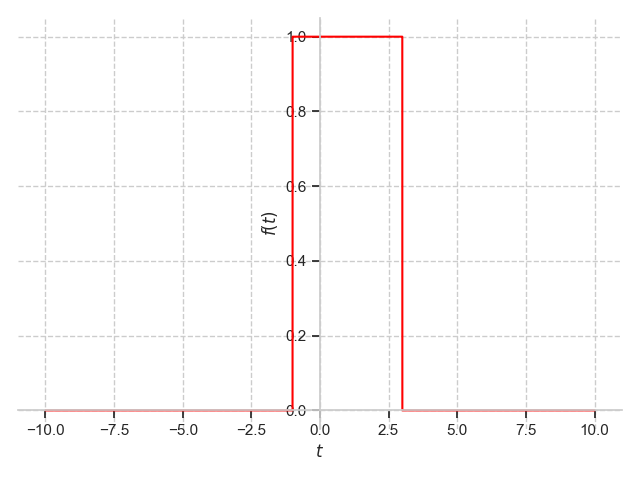
\includegraphics[width=\linewidth]{sh_m1_rectf_int12.png}
            \caption{$c=-1$}
            \label{fig:shrectf_1}
        \end{subfigure}
        \hfill
        \begin{subfigure}{0.3\textwidth}
            \centering
            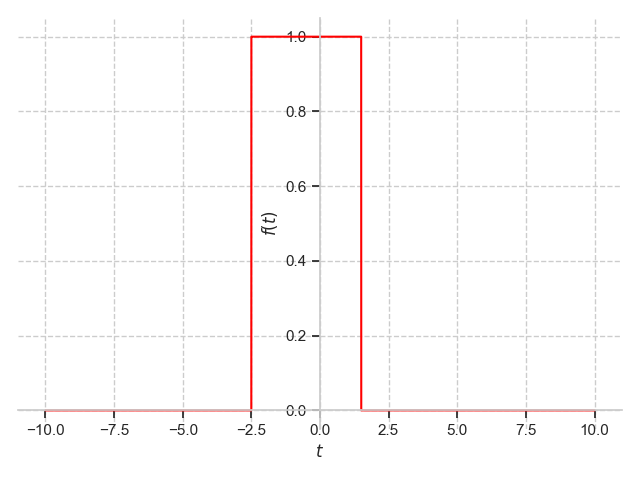
\includegraphics[width=\linewidth]{sh_zp5_rectf_int12.png}
            \caption{$c=0.5$}
            \label{fig:shrectf_2}
        \end{subfigure}
        \hfill
        \begin{subfigure}{0.3\textwidth}
            \centering
            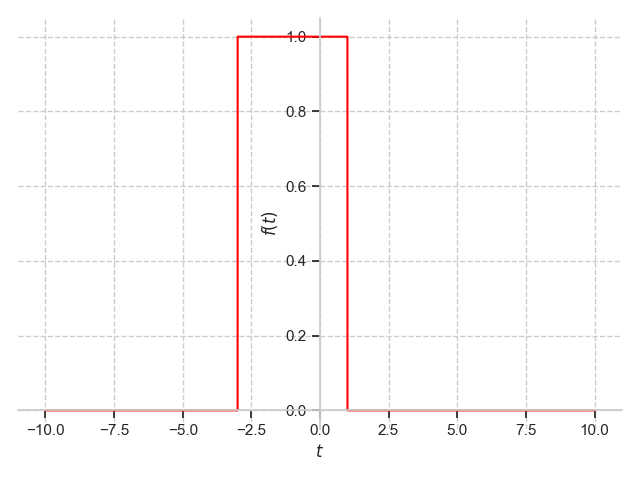
\includegraphics[width=\linewidth]{sh_1_rectf_int12.png}
            \caption{$c=1$}
            \label{fig:shrectf_3}
        \end{subfigure}
        \caption{Прямоугольные фукнции со смещением при различных значениях $c$}
        \label{fig:shrectfs}
    \end{figure}


    \noindent Построенные графики $\text{Re}\,{\hat{g}(\omega)}$ для нескольких значений параметра $c$ расположены ниже
    \begin{figure}[htbp]
        \centering
        \begin{subfigure}{0.3\textwidth}
            \centering
            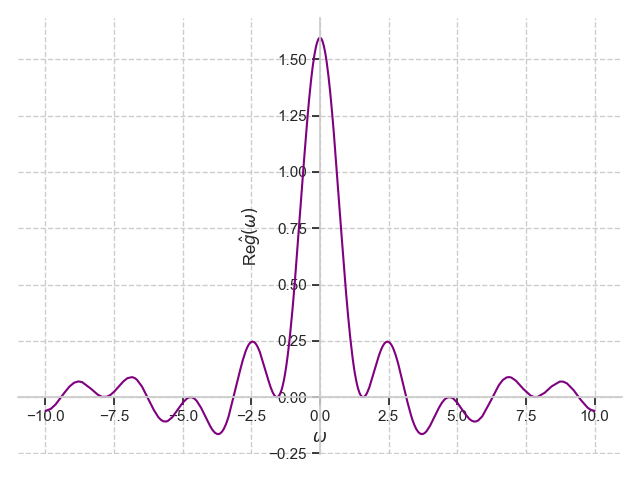
\includegraphics[width=\linewidth]{sh_m1_re_rectf_int12.png}
            \caption{$c=-1$}
            \label{fig:reshrectf_1}
        \end{subfigure}
        \hfill
        \begin{subfigure}{0.3\textwidth}
            \centering
            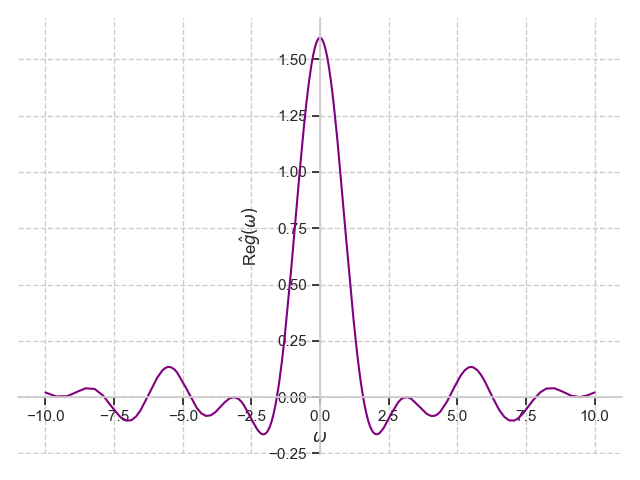
\includegraphics[width=\linewidth]{sh_zp5_re_rectf_int12.png}
            \caption{$c=0.5$}
            \label{fig:reshrectf_2}
        \end{subfigure}
        \hfill
        \begin{subfigure}{0.3\textwidth}
            \centering
            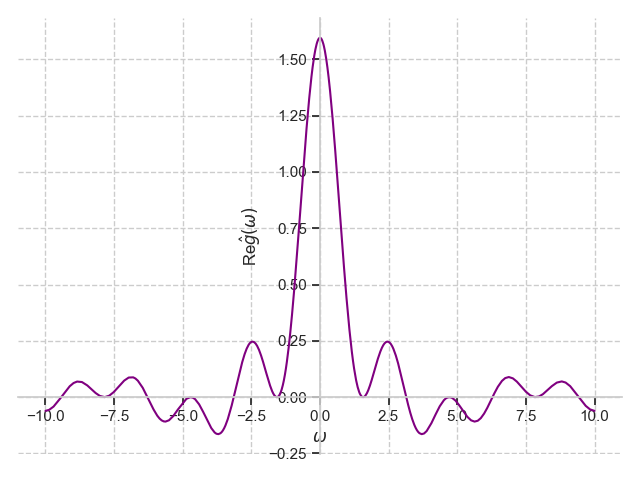
\includegraphics[width=\linewidth]{sh_1_re_rectf_int12.png}
            \caption{$c=1$}
            \label{fig:reshrectf_3}
        \end{subfigure}
        \caption{Действительные части Фурье-образов прямоугольных фукнций со смещением при различных значениях параметра $c$}
        \label{fig:reshrectfs}
    \end{figure}


    \noindent Построенные графики $\text{Im}\,{\hat{g}(\omega)}$ для нескольких значений параметра $c$ расположены ниже
    \begin{figure}[htbp]
        \centering
        \begin{subfigure}{0.3\textwidth}
            \centering
            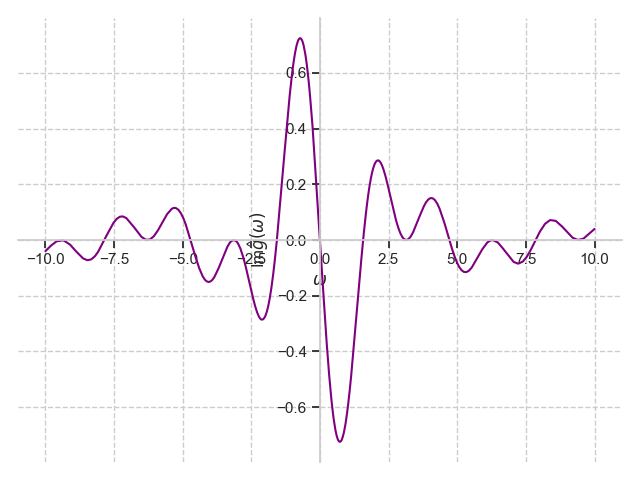
\includegraphics[width=\linewidth]{sh_m1_im_rectf_int12.png}
            \caption{$c=-1$}
            \label{fig:imshrectf_1}
        \end{subfigure}
        \hfill
        \begin{subfigure}{0.3\textwidth}
            \centering
            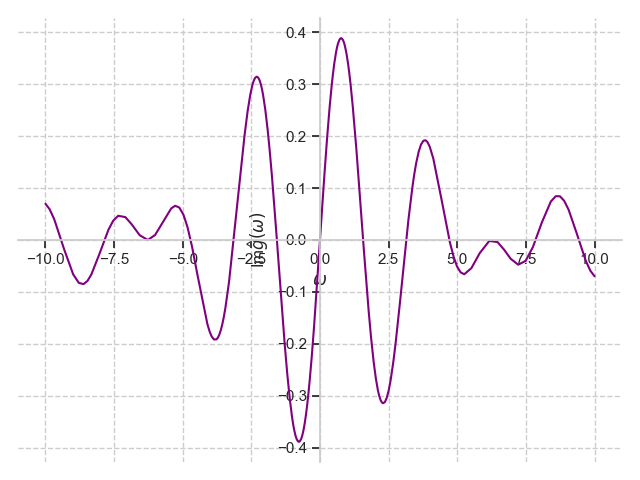
\includegraphics[width=\linewidth]{sh_zp5_im_rectf_int12.png}
            \caption{$c=0.5$}
            \label{fig:imshrectf_2}
        \end{subfigure}
        \hfill
        \begin{subfigure}{0.3\textwidth}
            \centering
            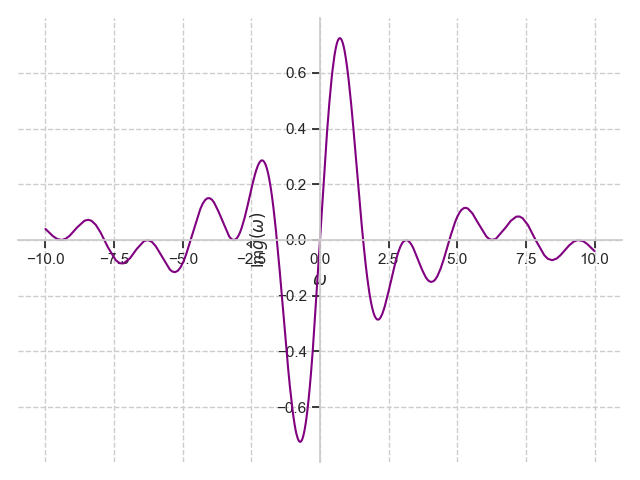
\includegraphics[width=\linewidth]{sh_1_im_rectf_int12.png}
            \caption{$c=1$}
            \label{fig:imshrectf_3}
        \end{subfigure}
        \caption{Мнимые части Фурье-образов прямоугольных фукнций со смещением при различных значениях параметра $c$}
        \label{fig:imshrectfs}
    \end{figure}


    \noindent Построенные графики $|\hat{g}(\omega)|$ для нескольких значений параметра $c$ расположены ниже
    \begin{figure}[htbp]
        \centering
        \begin{subfigure}{0.3\textwidth}
            \centering
            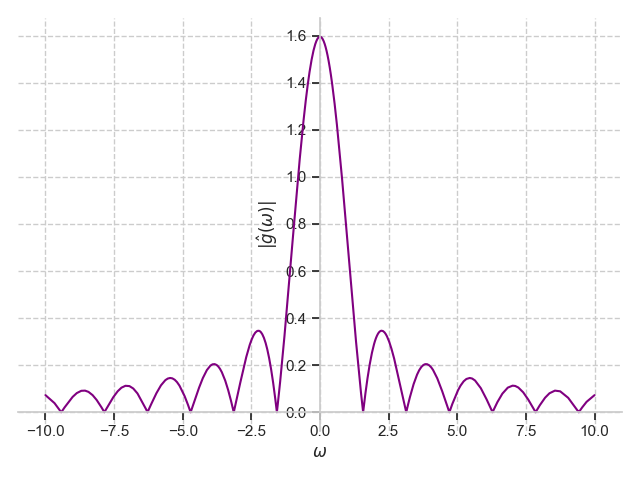
\includegraphics[width=\linewidth]{sh_m1_abs_rectf_int12.png}
            \caption{$c=-1$}
            \label{fig:absshrectf_1}
        \end{subfigure}
        \hfill
        \begin{subfigure}{0.3\textwidth}
            \centering
            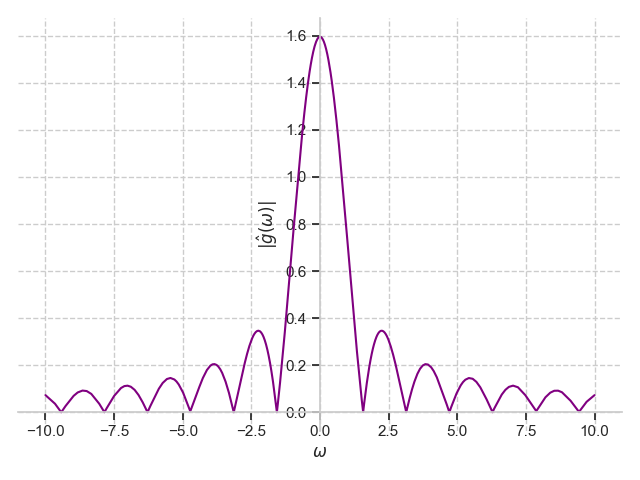
\includegraphics[width=\linewidth]{sh_zp5_abs_rectf_int12.png}
            \caption{$c=0.5$}
            \label{fig:absshrectf_2}
        \end{subfigure}
        \hfill
        \begin{subfigure}{0.3\textwidth}
            \centering
            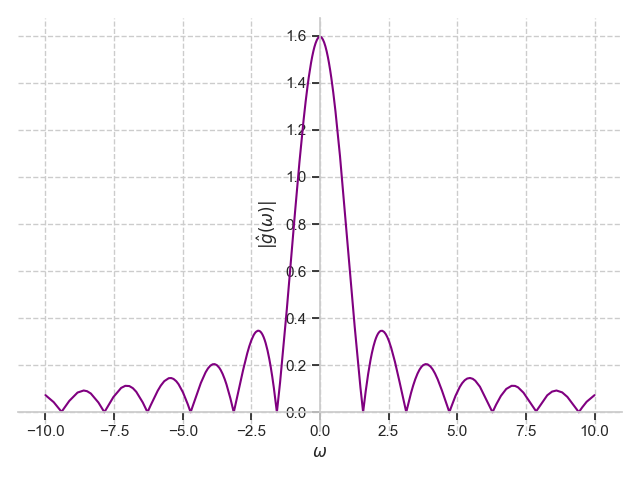
\includegraphics[width=\linewidth]{sh_1_abs_rectf_int12.png}
            \caption{$c=1$}
            \label{fig:absshrectf_3}
        \end{subfigure}
        \caption{Модули Фурье-образов прямоугольных фукнций со смещением при различных значениях параметра $c$}
        \label{fig:absshrectfs}
    \end{figure}


    % анализ влияния параметра c на функцию и Фурье-образ


    \section{Задание 3. Музыкальное}
    \noindent Для выполнения задания с представленного \href{https://drive.google.com/drive/folders/14lwzvV84uXtyuXXspoYUSf-VdR52t0sE}{гугл-диска}
    выбран аккорд номер 26


    \noindent Для считывания аудиозаписи в список используется библиотека librosa. В переменную y запишутся значения амплитуд аудиосигнала,
    в переменной sr будет частота дискретизации аудиосигнала, а t -- список временных отсчетов в секундах, соответствующий каждой амплитуде в списке y.
    На строках 15-17 показан пример использования метода. Указывается путь к mp3 файлу в переменной audio\_{file} и в переменной select\_{channel} хранится номер
    нужного звукового канала -- выбран первый канал. Аудиозапись длится 4 секунды, последняя из которых вырезана на 19-20 строках, так как не несет в себе
    важной информации, аккорд заканчивается раньше
    \begin{lstlisting}[label=mp3load, caption=Программа для считывания аудиозаписи в список]
    from librosa import load
    from numpy import linspace

    def get_y_sr_t(audio_file: str, select_channel: int):
        y, sr = load(audio_file)
    
        if select_channel >= y.ndim:
            select_channel = 0
    
        y = y[:, select_channel] if y.ndim > 1 else y
        t = linspace(0, len(y) / sr, len(y))
    
        return y, sr, t

    audio_file = 'fm_lab2/chord/chord26.mp3'
    select_channel = 0
    y, sr, t = get_y_sr_t(audio_file, select_channel)

    y = y[:3 * sr]
    t = t[:3 * sr]
    \end{lstlisting}


    \noindent Программа ниже построит график аудиозаписи $f(t)$
    \begin{lstlisting}[label=, caption=Программа для построения функции $f(t)$ аудиозаписи]
    import matplotlib.pyplot as plt

    def build_audio_f_t(t, y, clr=None):
        if (clr != None):
            plt.plot(t, y, color=clr)
        else:
            plt.plot(t, y)
    
        plt.xlabel(r'$t$')
        plt.ylabel(r'$f(t)$')
        plt.grid(True)
        plt.show()

    f_t_clr = colors_strs[0]
    build_audio_f_t(t, y, f_t_clr)
    \end{lstlisting}


    \noindent Результат выполнения программы для считанной в список аудиозаписи
    \begin{figure}[!htb]
        \centering
        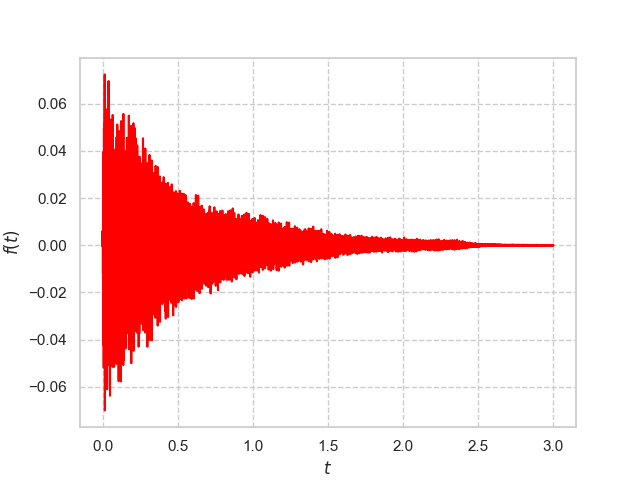
\includegraphics[scale=0.5]{f_t.png}
        \captionsetup{skip=0pt}
        \caption{График $f(t)$ аудиозаписи}
        \label{Рис:15}
    \end{figure}


    \noindent С помощью численного интегрирования trapz из библиотеки numpy найден Фурье-образ $\hat{f}(\nu)$
    по частотам freqs и записан в список ampls. Пример использования расположен на 11 строке
    \begin{lstlisting}[label=fimgmp3, caption=Программа для нахождения Фурье-образа аудиозаписи]
    def find_freqs_ampls(t, y, sr):
        freqs = linspace(0, sr / 2, len(y) // 2)
        ampls = []
    
        for freq in freqs:
            int = trapz(y * exp(-1j * 2 * pi * freq * t), t)
            ampls.append(abs(int))
    
        return freqs, ampls

    freqs, ampls = find_freqs_ampls(t, y, sr)
    \end{lstlisting}


    \noindent Программа ниже построит график $|\hat{f}(\nu)|$. Пример использования расположен на 17-24 строках
    \begin{lstlisting}[label=f_v_mp3, caption=Программа для построения графика $|\hat{f}(\nu)|$ аудиозаписи]
    def build_audio_f_v(freqs, ampls, start=None, stop=None, step=None, fz1=None, fz2=None, clr=None):
        if ((fz1 != None) and (fz2 != None)):
            plt.figure(figsize=(fz1, fz2))

        if (clr != None):
            plt.plot(freqs, ampls, color=clr)
        else:
            plt.plot(freqs, ampls)

        plt.xlabel(r'$\nu$')
        plt.ylabel(r'$\left|\hat{f}\left(\nu\right)\right|$')
        plt.grid(True)
        if ((start != None) and (stop != None and stop != 0) and (step != None and step != 0)):
            plt.xticks(arange(start, stop, step))
        plt.show()

    start = 0
    stop = 10001
    step = 1000
    figsize1 = 10
    figsize2 = 6
    f_v_clr = colors_strs[1]

    build_audio_f_v(freqs, ampls, start=start, stop=stop, step=step,
                    fz1=figsize1, fz2=figsize2, clr=f_v_clr)
    \end{lstlisting}


    \noindent Построенный график $|\hat{f}(\nu)|$ расположен ниже
    \begin{figure}[!htb]
        \centering
        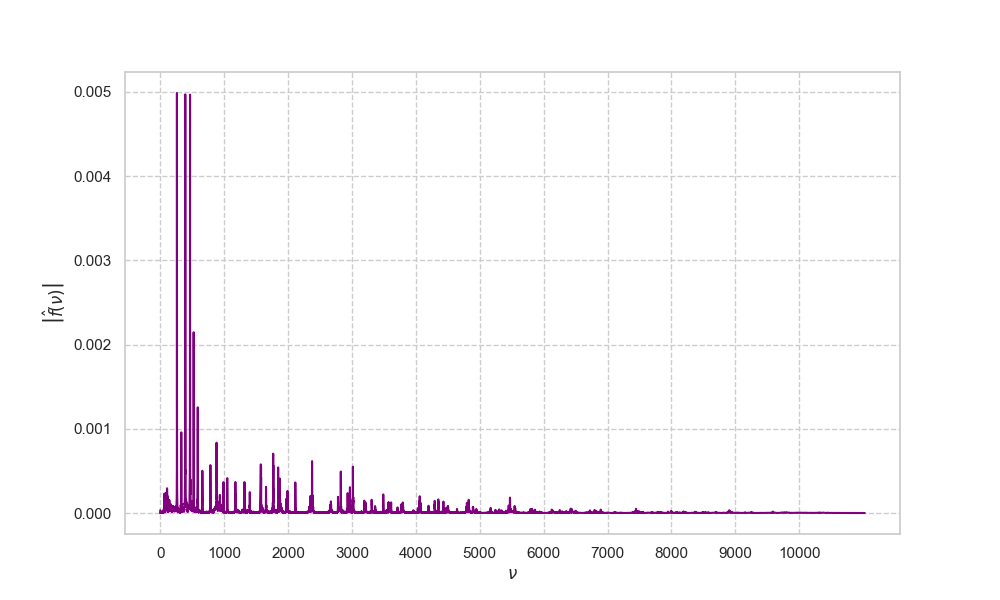
\includegraphics[scale=0.5]{f_v.png}
        \captionsetup{skip=0pt}
        \caption{График $|\hat{f}(\nu)|$ аудиозаписи}
        \label{Рис:16}
    \end{figure}


    \noindent Так как на большом интервале частот трудно разобрать из каких нот состоит аккорд,
    нужен код для уменьшения интервала и шага без потери данных или искажения графиков
    \begin{lstlisting}[label=f_v_1k, caption={Программа для изменения интервала частот и амплитуд}]
    r_start = 0
    r_end = 1000
        
    start_idx = next(idx for idx, freq in enumerate(freqs) if freq >= r_start)
    end_idx = next(idx for idx, freq in enumerate(freqs) if freq > r_end)
        
    r_ampls = ampls[start_idx:end_idx]
    r_freqs = freqs[start_idx:end_idx]
    r_step = 20

    build_audio_f_v(r_freqs, r_ampls, start=r_start, stop=r_end, step=r_step, fz1=figsize1, fz2=figsize2, clr=f_v_clr)
    \end{lstlisting}
    

    \noindent Построенный график $|\hat{f}(\nu)|$ на интервале частот от $0$ до $1000$
    \begin{figure}[!htb]
        \centering
        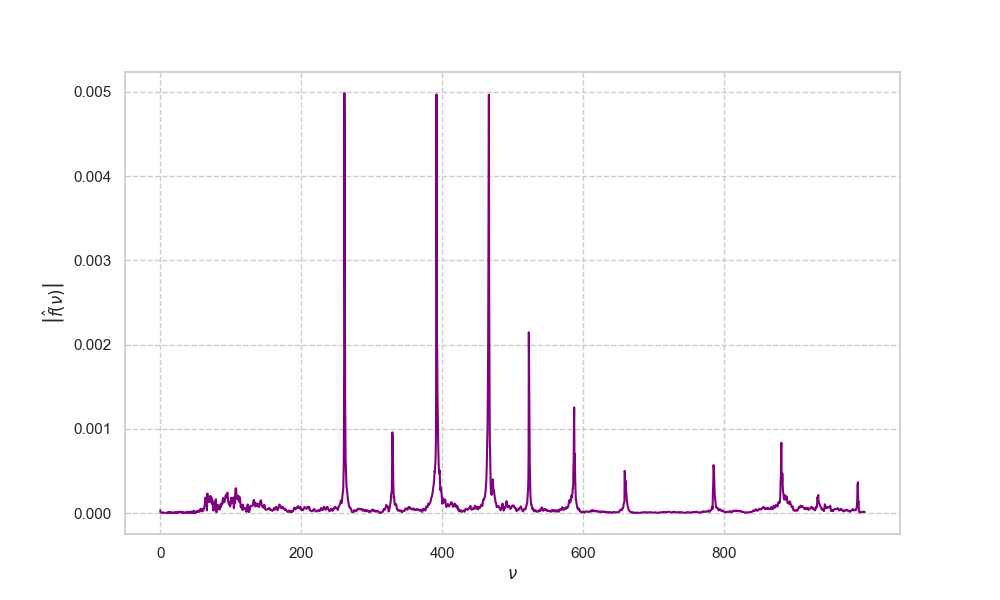
\includegraphics[scale=0.5]{f_v_reduced_1k.png}
        \captionsetup{skip=0pt}
        \caption{График $|\hat{f}(\nu)|$ аудиозаписи на интервале частот от 0 до 1000}
        \label{Рис:17}
    \end{figure}


    \noindent Для точности определения нот построен график $|\hat{f}(\nu)|$ на интервале частот от $200$ до $500$
    \begin{figure}[!htb]
        \centering
        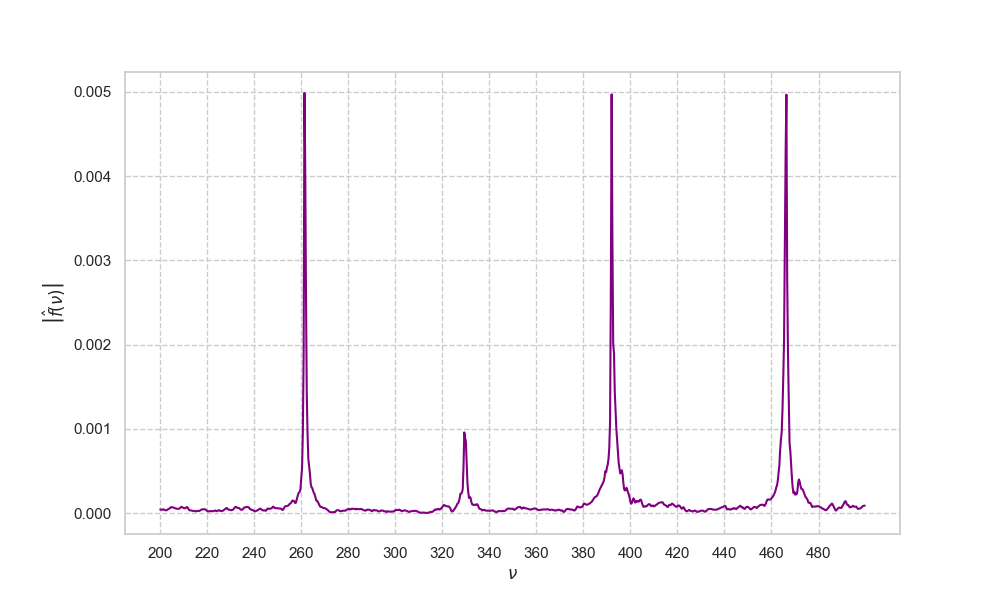
\includegraphics[scale=0.5]{f_v_reduced_200_to_500.png}
        \captionsetup{skip=0pt}
        \caption{График $|\hat{f}(\nu)|$ аудиозаписи на интервале частот от 200 до 500}
        \label{Рис:18}
    \end{figure}


    % анализ графика, проверить ноты


    \noindent Исходя из графика на уменьшенном интервале частот определены ноты: первая До, первая Соль, первая Ля диез
\end{document}